\documentclass[11pt]{article}
\usepackage{graphicx}
\usepackage{booktabs}
\usepackage{float}
\usepackage{caption}
\usepackage{geometry}
\geometry{margin=1in}
\usepackage{setspace}
\onehalfspacing

\title{Problem Set 5 -- Munson \\ ECON 833: Computational Economics}
\author{David Munson}
\date{\today}

\begin{document}
\maketitle

\section{Research Question}
This project investigates how changes in the Federal Funds Rate (FFR) affect market-based inflation expectations, measured by the 5-Year Breakeven Inflation Rate (T5YIE). The Federal Reserve sets the FFR as a key monetary policy instrument; studying its relationship with inflation expectations helps evaluate policy credibility and effectiveness.  I suspect the relationship is complex due to the endogenous nature of policy decisions and expectations formation.

\section{Data}
Data are sourced from FRED. The key series are:
\begin{itemize}
  \item \textbf{FEDFUNDS:} Effective Federal Funds Rate (monthly)
  \item \textbf{T5YIE:} 5-Year Breakeven Inflation Rate
  \item \textbf{CPIAUCSL:} Consumer Price Index for All Urban Consumers (used to compute CPI YoY)
  \item \textbf{UNRATE:} Unemployment Rate
\end{itemize}

\section{Visualizations}
\begin{figure}[H]
  \centering
  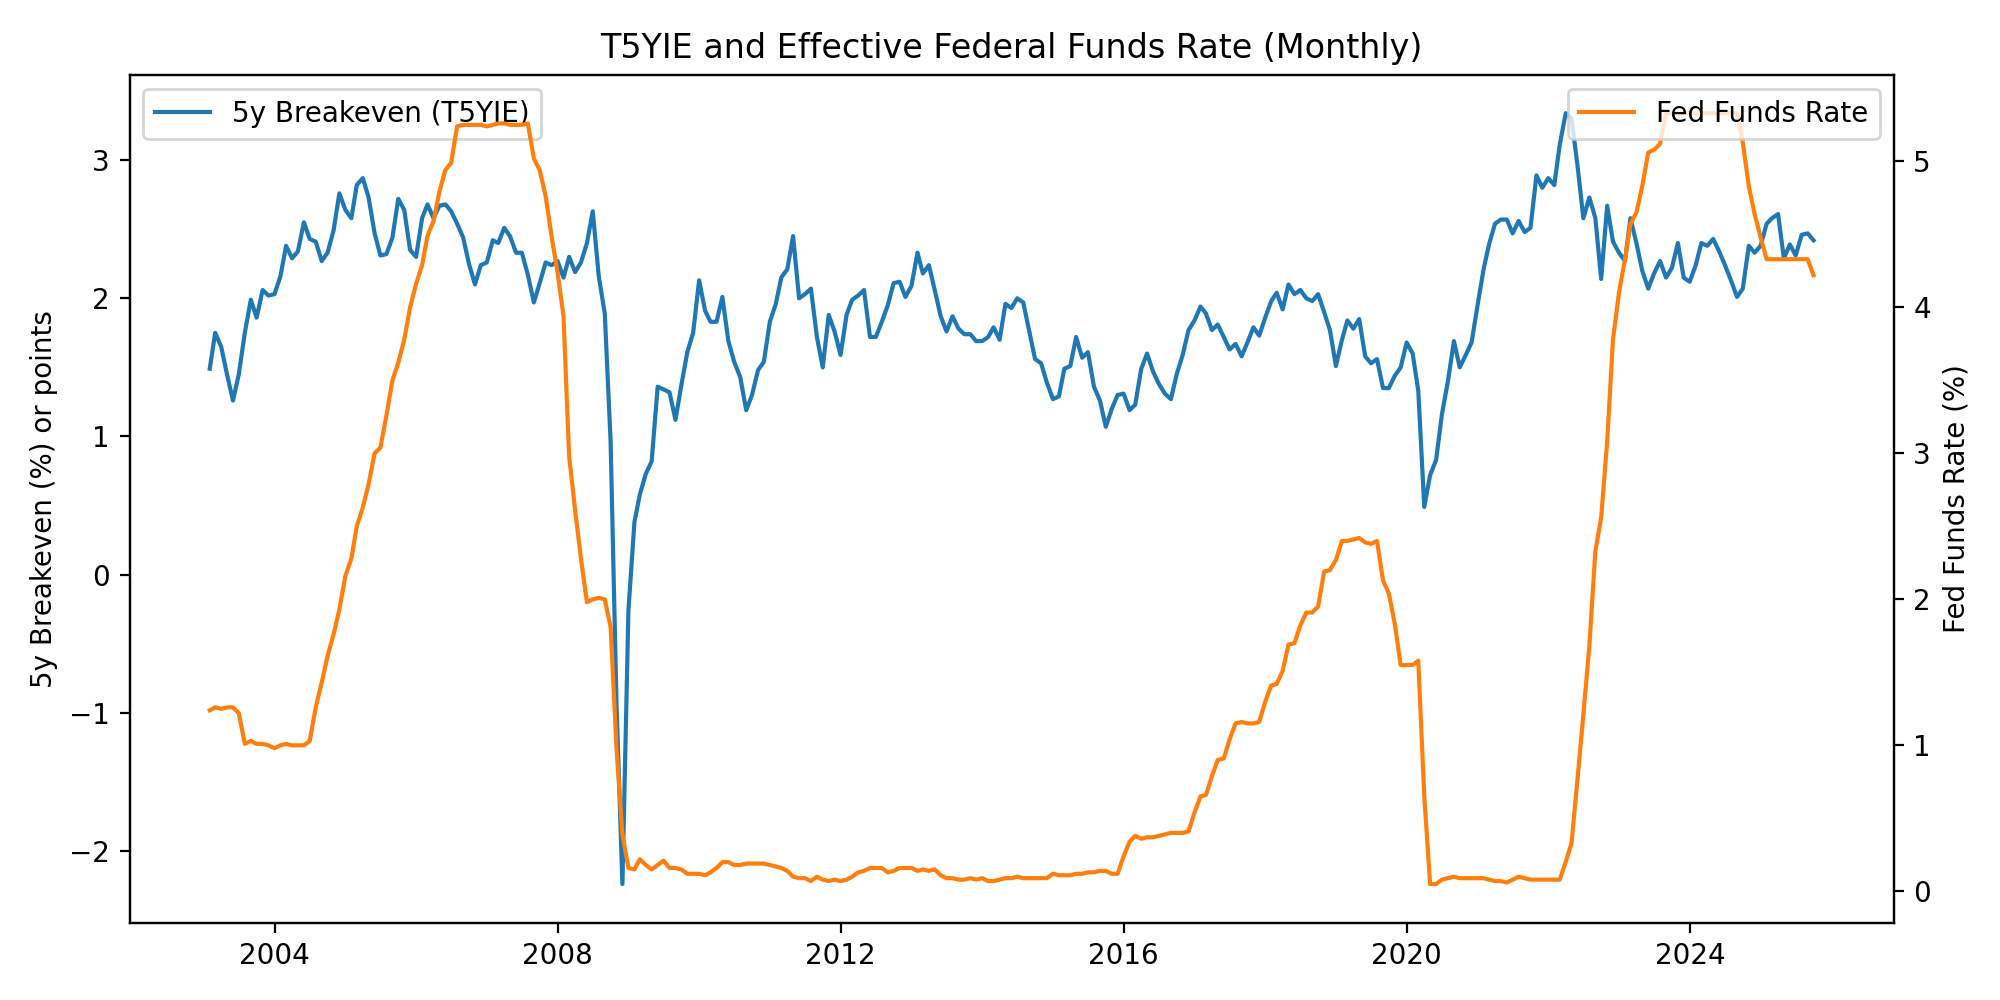
\includegraphics[width=0.9\textwidth]{images/fig1_timeseries.png}
  \caption{Time series: 5-year breakeven inflation (left axis) and Federal Funds Rate (right axis).}
\end{figure}

\begin{figure}[H]
  \centering
  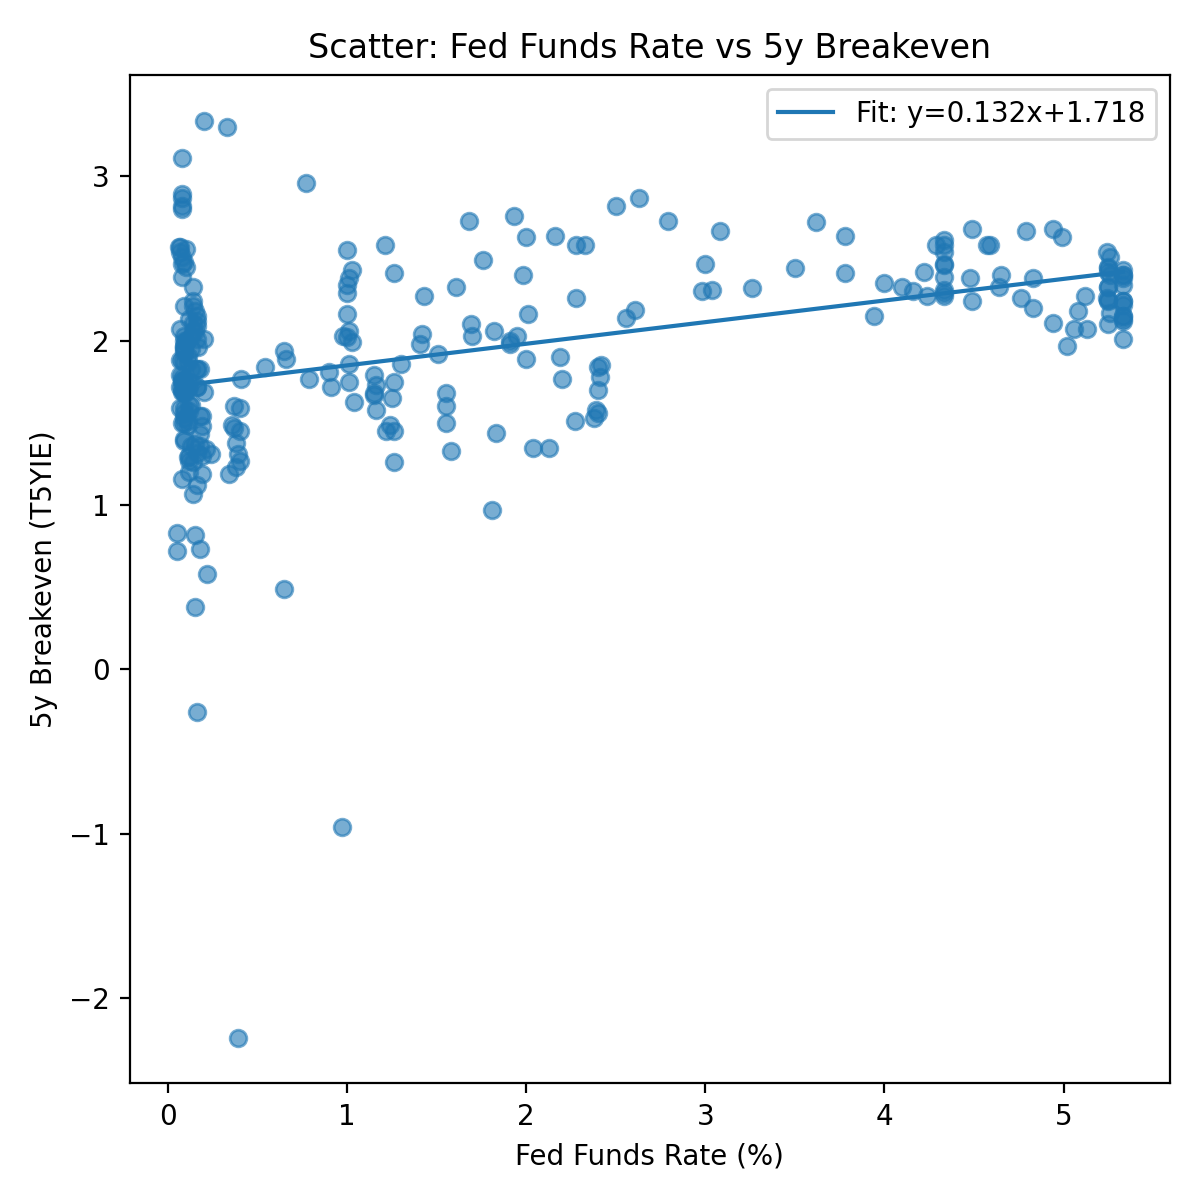
\includegraphics[width=0.7\textwidth]{images/fig2_scatter.png}
  \caption{Scatter plot of Fed Funds Rate vs 5-year breakeven inflation with fitted linear trend.}
\end{figure}

\begin{figure}[H]
  \centering
  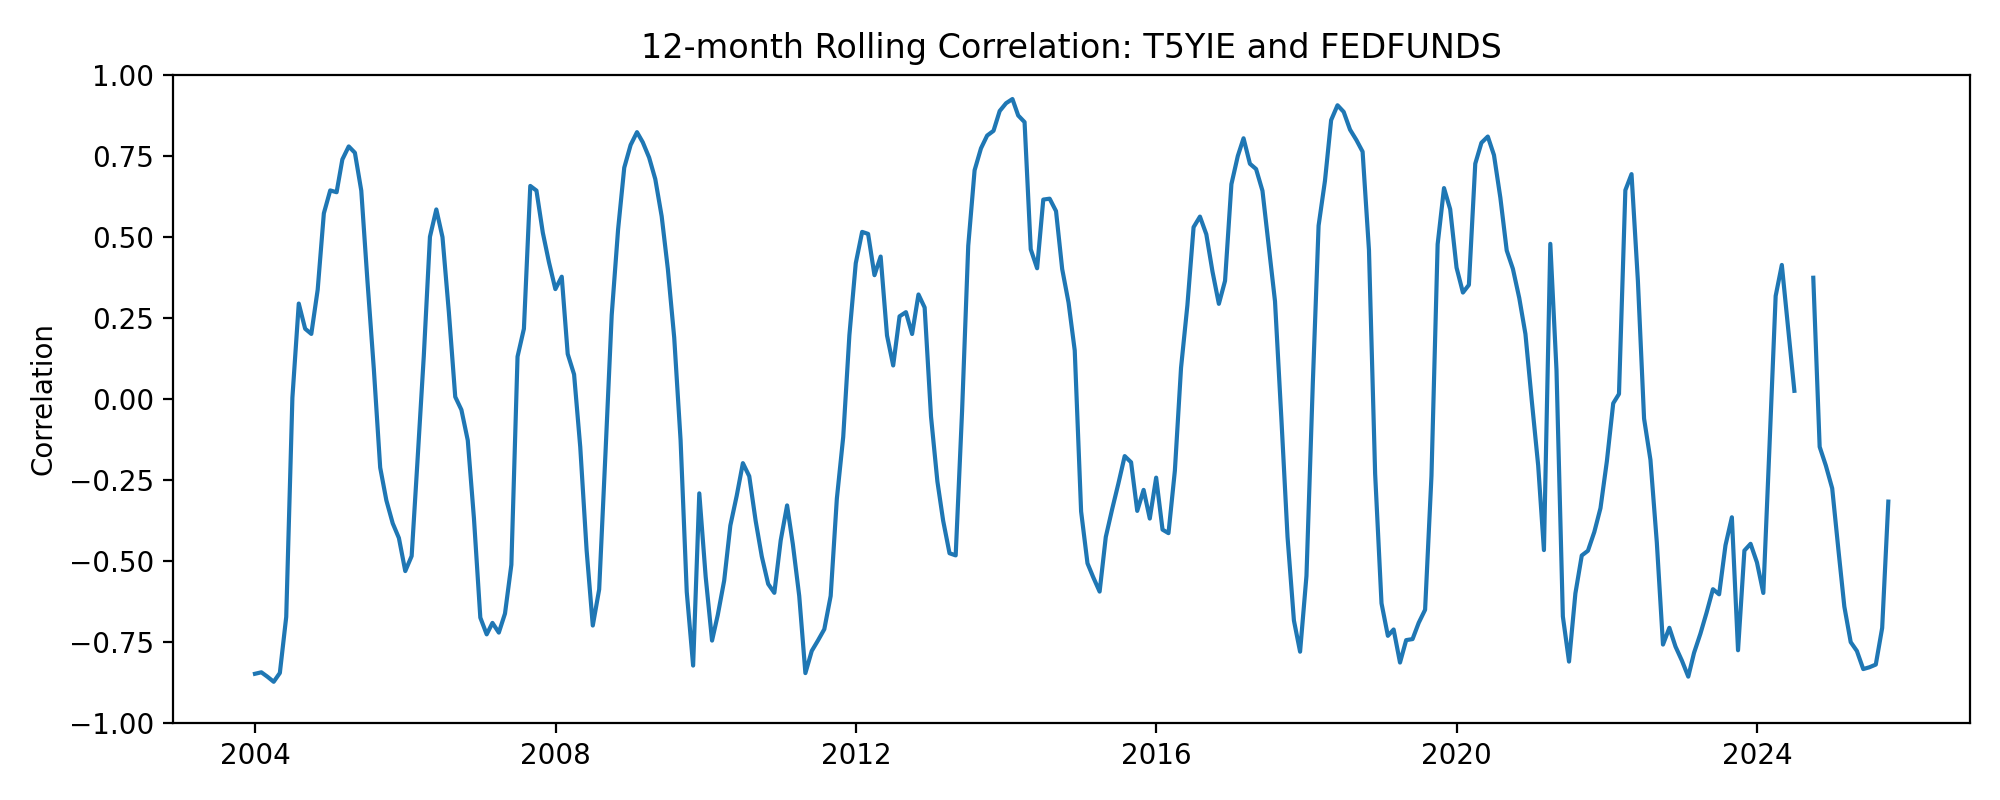
\includegraphics[width=0.9\textwidth]{images/fig3_rollingcorr.png}
  \caption{12-month rolling correlation between the Fed Funds Rate and the 5-year breakeven.}
\end{figure}

\section{Econometric Results}
We estimate three OLS specifications:

\begin{itemize}
  \item \textbf{Model 1:} $T5YIE_t = \alpha + \beta_1\, FEDFUNDS_t + \epsilon_t$
  \item \textbf{Model 2:} adds a one-period lag of the Fed Funds Rate: $FEDFUNDS_{t-1}$
  \item \textbf{Model 3:} controls for macro conditions: CPI YoY and unemployment (UNRATE)
\end{itemize}

\vspace{6pt}
\noindent\textbf{Regression table (coefficients with standard errors in parentheses):}

\begin{table}[H]
\centering
\caption{OLS estimates: 5-year breakeven (T5YIE) on policy and controls}
\label{tab:results}
\begin{tabular}{lccc}
\toprule
 & \textbf{Model 1} & \textbf{Model 2} & \textbf{Model 3} \\
\midrule
\textbf{const} & 1.7261 (0.0467) & 1.7256 (0.0418) & 1.3207 (0.1422) \\
\textbf{FEDFUNDS} & 0.1305 (0.0180) & 1.5787 (0.1803) & 0.0778 (0.0183) \\
\textbf{FEDFUNDS\_L1} & -- & -1.4587 (0.1809) & -- \\
\textbf{CPI\_YoY} & -- & -- & 0.1823 (0.0169) \\
\textbf{UNRATE} & -- & -- & 0.0044 (0.0178) \\
\midrule
$R^2$ & 0.1698 & 0.3375 & 0.4455 \\
\bottomrule
\end{tabular}
\end{table}

\section{Discussion}
The baseline regression (Model 1) yields a small positive coefficient on the Federal Funds Rate (0.1305), meaning that same period increases in the Fed Funds Rate are associated with slightly higher 5-year breakeven inflation in the sample. At first glance this is not what one would expect if tightening monetary policy led the market to expect lower inflation moving forward.

Model 2, includes a one-month lag of the Fed Funds Rate, shows a strong positive same period coefficient (1.5787) and a negative lagged coefficient (-1.4587), which roughly offset. This pattern suggests timing dynamics: part of the short-run positive association may reflect the Fed reacting to rising inflation expectations (policy response), while the negative lag indicates that policy may reduce expectations with some delay.

Model 3 introduces controls for CPI year-over-year inflation and unemployment. The FEDFUNDS coefficient becomes smaller (0.0778) and CPI\_YoY enters positively and significantly (0.1823). The pattern again points to endogeneity with the Fed raising rates in response to rising inflation expectations.

\bigskip

\end{document}
